\documentclass[a4paper]{article}

\usepackage{fullpage} % Package to use full page
\usepackage{parskip} % Package to tweak paragraph skipping
\usepackage{tikz} % Package for drawing
\usepackage{amsmath, amssymb}
\usepackage[amsthm, thmmarks]{ntheorem}
\usepackage{hyperref}
\usepackage[utf8]{inputenc}
\usepackage[english]{babel}

\theoremstyle{break}

\newtheorem{theorem}{Theorem}[section]
\newtheorem{definition}{Definition}[section]
\newtheorem{corollary}{Corollary}[theorem]
\newtheorem{lemma}[theorem]{Lemma}



\newcommand{\R}{\mathbb{R}}
\newcommand{\Nu}{\mathcal{N}}
\newcommand{\Ra}{\mathcal{R}}
\newcommand{\Mat}[2]{\mathbb{M}(#1, #2)}

\newcommand{\pll}{\parallel}

\title{Mathematics behind Machine Learning Algorithms}
\author{Hubert Beres}
\date{2018/01/08}

\begin{document}

\maketitle

\section{Introduction}
\subsection{Conventions}
\begin{enumerate}
    \item Vectors are by default column vectors,
    \item Matrices are real,
    \item Orthogonal vectors are denoted by $ v \perp w$
    \item $\Nu(H)$ resp. $\Ra(H)$ denote the null space resp. the range of a matrix $H$, 
\end{enumerate}
\subsection{Problem overview}
\begin{enumerate}
    \item Recently we face many problems where objective is to guess a function of multiple variables (features) based on multiple examples (values at particular points)
    \item discuss high computational complexity and 
    \item define basic ML terminology: test set, label, (parametric) model, error function, test error, search space for function parameters
    \item particular case is Multiple Regression
    \item argue why small parameter values are generally considered better (over-fitting issues)

\end{enumerate}

\begin{definition}[Multiple Regression]
    Given a real-valued $ n \times m$ matrix $T$ and a n-vector $l$ a Multiple Regression Model is a linear map $f \in \mathcal{L} ( \R ^n, \R)$ represented by a $ 1 \times n$ matrix $w$ such that
    \begin{equation}
        \| T w - l \| = \inf\limits_{x \in \R^n} \| T x - l \|
    \end{equation}
\end{definition}    

\section{Optimisation tools}
Goal: solving for Multiple Regression
Error function: squared residuals
Model: linear map

\subsection{Moore-Penrose pseudoinverse}
\subsubsection{Facts from Linear Algebra}

\begin{theorem}[Orthogonal decomposition]
    Let $z \in \R^n$ and $V \subset \R^n$ be a vector subspace. Then
    \begin{enumerate}
        \item We write $z \perp V$ when $ z \perp x$ for every $x \in V$.
        \item Orthogonal complement of $V$ is $V^\perp := \{ v \in \R^n : v \perp V\}$
        \item There exist unique $z_\perp \in V^\perp$ and $z_\pll \in V$ such that  
            \begin{equation}
                z = z_\perp + z_\pll
            \end{equation}
        \item For any $y \in V$
        \begin{equation}
                \| z - y \| \geq \| z - z_\pll \|
        \end{equation}
        with strict inequality whenever $y \neq z_\pll$
    \end{enumerate}
\end{theorem}
\begin{proof}
    Proof of inequality.
\end{proof}

\begin{theorem}
    $\Nu(H) = \Ra^\perp(H^T)$ for any matrix $H \in \Mat{n}{m}$.
\end{theorem}

\begin{corollary}
\begin{enumerate}
    \item  $\Nu^\perp(H) = \Ra(H^T)$
    \item  For every vector $z \in R^n$ there exists unique decomposition $z = z_\Ra + z_\Nu$ where $z_\Ra \in \Ra(H)$ and $z_\Nu \in \Nu(H^T)$.
\end{enumerate}
\end{corollary}
\begin{proof}
    Full proof
\end{proof}

\begin{lemma}[Symmetric matrices]
\begin{enumerate}
    \item For symmetric matrix A $\Nu(A) = \Ra^\perp(A)$ and $\Nu^\perp(A) = \Ra(A)$
    \item Matrices of the form $H^T H$ and $H H^T$ are always symmetric,
    \item $\Ra(H) = \Ra(H H^T)$ and $\Ra(H^T) = \Ra(H^T H)$
\end{enumerate}
\end{lemma}

\subsection{Moore-Penrose pseudoinverse}

\begin{theorem}
\begin{enumerate}
    \item With $H$ as above and $z \in \R^n$ the set
        \begin{equation*}
        X := \{ x \in \R^n : \| z - H x \| = \inf\limits_{y \in \R^n} \| z - H y \| \}
        \end{equation*}
        is not empty, i.e. there is a vector $x$ minimising $\| z - H x \|$.
    \item There is a unique vector $\hat{x}$ with minimum norm in X.
    \item $\hat{x}$ is the unique vector in $\Ra(H^T)$ which satisfies $Hx = z_\Ra$ where $z_\Ra$ is a projection of z on $\Ra(H)$.
\end{enumerate}
\end{theorem}
\begin{proof}
    Full proof
\end{proof}

\begin{lemma}
    For any nonzero $\delta$ the matrix $H^T H + \delta^2 * I_m$ is invertible.
\end{lemma}
\begin{proof}
    Full proof.
\end{proof}

\begin{lemma}
    For a real symmetric matrix A, the below exists:
    \begin{equation}
        P_A = \lim_{\delta \to 0} A ( A + \delta I) ^-1
            = \lim_{\delta \to 0} ( A + \delta I) ^-1 A
    \end{equation}
    
\end{lemma}
\pagebreak
\section{Neural networks}
Key difference: non-linear model
Def. Activation function
Def. Activation bias

$H \in \Mat{n}{m}$
\subsection{Context and motivation}
A paragraph
\subsection{Definitions}
\subsection{Learning}












































\pagebreak
\section{Sample usage (from template)}

Differentiation is a concept of Mathematics studied in Calculus. There is an ongoing discussion as to who was the first to define differentiation: Leibniz or Newton \cite{bardi2006calculus}.

Differentiation allows for the calculation of the slope of the tangent of a curve at any given point as shown in Figure \ref{exampleplot}.

\begin{figure}[!htbp]
\begin{center}
\begin{tikzpicture}
\draw[domain=-2:2, color=blue] plot (\x, {1 - (\x)^2}) node[above = .5cm, right, color=blue] {$f(x)=1-x^2$};
\draw[domain=-2:2, color=red] plot(\x,-1 * \x + 1.25) node[above = .5cm, right, color=red] {Tangent at $x=.5$};
\draw [thick, ->] (-3,0) -- (3,0) node [above] {$x$};
\draw [thick, ->] (0,-3) -- (0,3) node [right] {$y$};
\node at (.5,.75) {\textbullet};
\end{tikzpicture}
\end{center}
\caption{The plot of $f(x)=1-x^2$ with a tangent at $x=.5$.}\label{exampleplot}
\end{figure}

Differentiation is now a technique taught to mathematics students throughout the world. In this document I will discuss some aspects of differentiation.

\section{Exploring the derivative using Sage}

The definition of the limit of $f(x)$ at $x=a$ denoted as $f'(a)$ is:

\begin{equation}
f'(a) = \lim_{h\to0}\frac{f(a+h)-f(a)}{h}
\end{equation}

The following code can be used in sage to give the above limit:

\begin{verbatim}
def illustrate(f, a):
    """
    Function to take a function and illustrate the limiting definition of a derivative at a given point.
    """
    lst = []
    for h in srange(.01, 3, .01):
    	lst.append([h,(f(a+h)-f(a))/h])
    return list_plot(lst, axes_labels=['$x$','$\\frac{f(%.02f+h)-f(%.02f)}{h}$' % (a,a)])
\end{verbatim}

\begin{figure}[!htbp]
\begin{center}
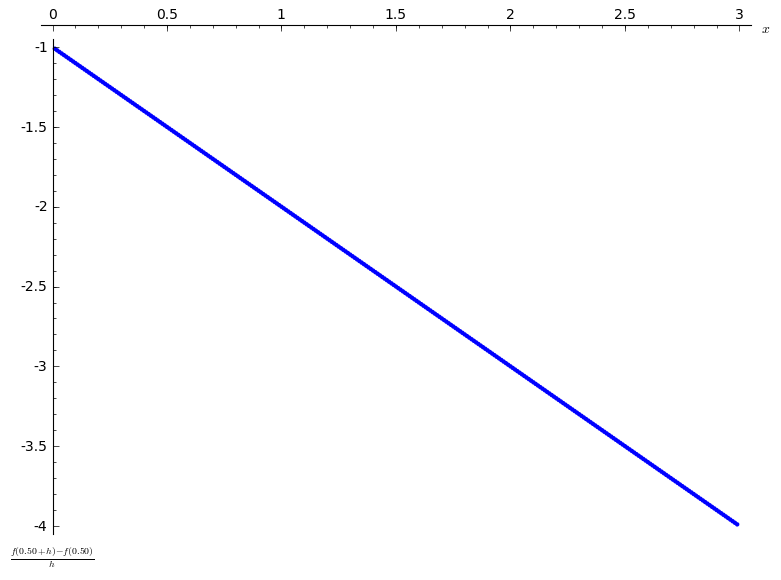
\includegraphics[width=8cm]{sage1.png}
\end{center}
\caption{The derivative of $f(x)=1-x^2$ at $x=.5$ converging to -1 as $h\to0$.}
\end{figure}

If we want to plot the tangent at a point $\alpha$ to a function we can use the following:

\begin{align}
y=&ax+b&&\text{(definition of a straight line)}\nonumber\\
  &f'(a)x+b&&\text{(definition of the derivative)}\nonumber\\
  &f'(a)x+f(a)-f'(a)a&&\text{(we know that the line intersects $f$ at $(a,f(a))$}\nonumber
\end{align}

We can combine this with the approach of the previous piece of code to see how the tangential line converges as the limiting definition of the derivative converges:

\begin{verbatim}
def convergetangentialline(f, a, x1, x2, nbrofplots=50, epsilon=.1):
    """
    Function to make a tangential line converge
    """
    clrs = rainbow(nbrofplots)
    k = 0
    h = epsilon
    p = plot(f, x, x1, x2)
    while k < nbrofplots:
        tangent(x) = fdash(f, a, h) * x + f(a) - fdash(f, a, h) * a
        p += plot(tangent(x), x, x1, x2, color=clrs[k])
        h += epsilon
        k += 1
    return p
\end{verbatim}

The plot shown in Figure \ref{lines} shows how the lines shown converge to the actual tangent to $1-x^2$ as $x=2$ (the red line is the `closest' curve).

\begin{figure}[!htbp]
\begin{center}
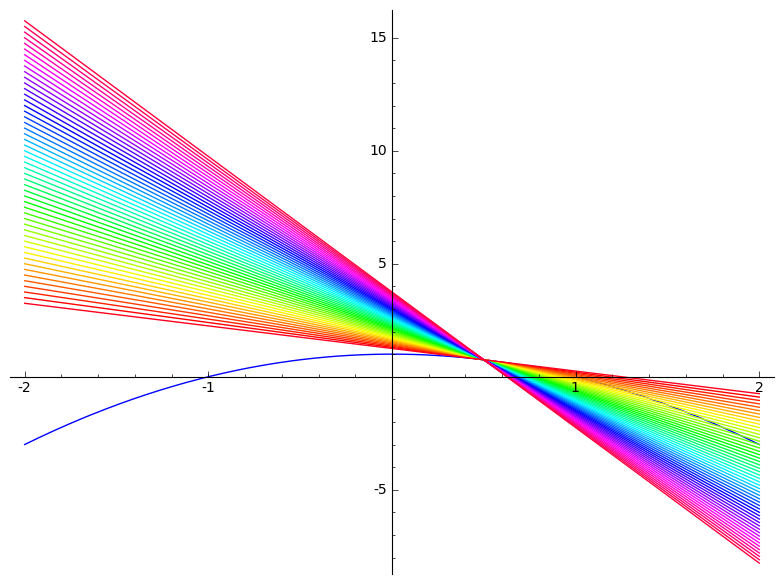
\includegraphics[width=8cm]{sage0.png}
\end{center}
\caption{Lines converging to the tangent curve as $h\to0$.}\label{lines}
\end{figure}

Note here that the last plot is given using the \textbf{real} definition of the derivative and not the approximation.

\section{Conclusions}

In this report I have explored the limiting definition of the limit showing how as $h\to 0$ we can visualise the derivative of a function. The code involved \url{https://sage.maths.cf.ac.uk/home/pub/18/} uses the differentiation capabilities of Sage but also the plotting abilities.

There are various other aspects that could be explored such as symbolic differentiation rules. For example:

$$\frac{dx^n}{dx}=(n+1)x^{n}\text{ if }x\ne-1$$

Furthermore it is interesting to not that there exists some functions that \textbf{are not} differentiable at a point such as the function $f(x)=\sin(1/x)$ which is not differentiable at $x=0$. A plot of this function is shown in Figure \ref{notdiff}.

\begin{figure}[!htbp]
\begin{center}
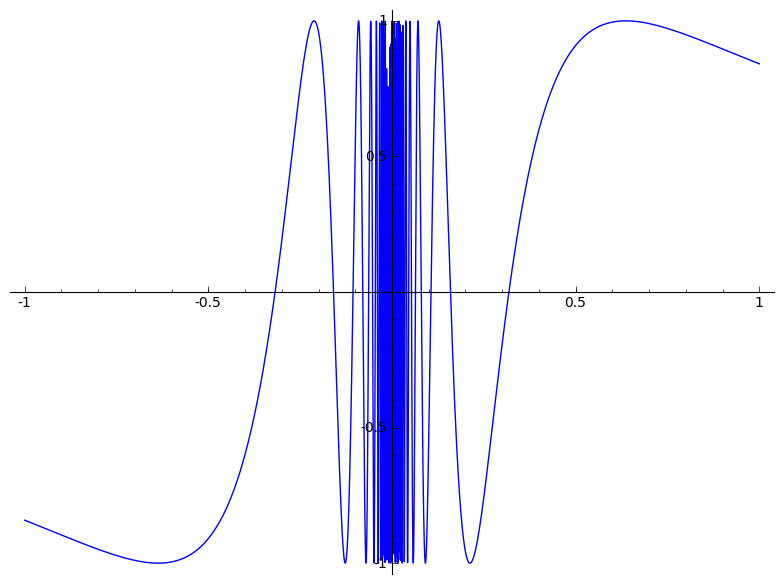
\includegraphics[width=8cm]{sage2.png}
\end{center}
\caption{None differentiable function at $x=0$.}\label{notdiff}
\end{figure}


\bibliographystyle{plain}
\bibliography{bibliography.bib}
\end{document}